\documentclass[11pt,a4paper]{article}
\usepackage{multirow}
\usepackage[utf8]{inputenc}
\usepackage[italian]{babel}
\usepackage[margin=2.5cm]{geometry}
\usepackage{graphicx}
\usepackage{amsmath}
\usepackage{hyperref}
\usepackage{float}
\usepackage{tikz}
\usetikzlibrary{automata, positioning, arrows.meta}
\usepackage{pgfplots}
\pgfplotsset{compat=1.18}

\usepackage{listings}
\usepackage{xcolor}

% Definizione colori per il codice sorgente
\definecolor{codegreen}{rgb}{0,0.6,0}
\definecolor{codegray}{rgb}{0.5,0.5,0.5}
\definecolor{codepurple}{rgb}{0.58,0,0.82}
\definecolor{backcolour}{rgb}{0.96,0.96,0.96}

\lstdefinestyle{pystyle}{
    backgroundcolor=\color{backcolour},   
    commentstyle=\color{codegreen}\itshape,
    keywordstyle=\color{blue}\bfseries,
    numberstyle=\tiny\color{codegray},
    stringstyle=\color{codepurple},
    basicstyle=\ttfamily\footnotesize,
    breakatwhitespace=false,         
    breaklines=true,                 
    captionpos=b,                    
    keepspaces=true,                 
    numbers=left,                    
    numbersep=5pt,                  
    showspaces=false,                
    showstringspaces=false,
    showtabs=false,                  
    tabsize=4
}
\lstset{style=pystyle}

\definecolor{linkcolor}{HTML}{0006b1}

\hypersetup{
    colorlinks=true,
    linkcolor=linkcolor,
    filecolor=transparent,      
    urlcolor=linkcolor
    }

\title{\textbf{Relazione di Progetto: Sistema Multi-Agente per il Recupero di Oggetti in una Rete di Magazzini}}
\author{Antonio Rosano, Angelo Spadola, Marco Spampinato}
\date{}

\begin{document}

\maketitle

Link alla repository: \href{https://github.com/marcospampi/progetto-ai-swarm}{GitHub - AI Swarm Project}.

\section{Introduzione e Definizione del Problema}
Il presente elaborato si presenta come relazione di progetto di un modello di simulazione basato su un Sistema Multi-Agente. Lo scopo del sistema realizzato è coordinare una flotta di agenti robotici autonomi incaricati di ricercare, recuperare e posizionare un insieme di oggetti dispersi in una vasta area logistica composta da una rete di magazzini.

\vspace{0.3cm}
\noindent
Il dominio operativo è modellato come una griglia bidimensionale statica. Rispetto alle specifiche di base, è stata rimossa la conoscenza pregressa sul numero e sulla collocazione dei magazzini, al fine di introdurre un maggiore grado di realismo e complessità. Partendo dalla cella in alto a sinistra di coordinate [0,0], la flotta ha il compito di esplorare l'area alla cieca, individuando dinamicamente sia i punti di drop-off (magazzini) che gli oggetti da recuperare, costruendo e aggiornando la propria mappa locale in tempo reale.

\vspace{0.3cm}
\noindent
L'efficienza del modello algoritmico viene valutata in base alla sua capacità di ottimizzare simultaneamente tre metriche fondamentali:
\begin{enumerate}
    \item Massimizzare il numero di oggetti rilevati e correttamente posizionati all'interno del magazzino.
    \item Minimizzare il tempo totale di recupero.
    \item Minimizzare l'energia media consumata dagli agenti durante le operazioni esplorative e di trasporto.
\end{enumerate}

\section{Software realizzato}
Il modello di simulazione proposto ha sua implementazione realizzata usando il linguaggio di programmazione \textit{Python 3} e le relative librerie \textit{numpy} per la manipolazione di array n-dimensionali, \textit{pandas} per la manipolazione dei dati dei risultati, \textit{matplotlib} e \textit{rich} rispettivamente per la visualizzazione della simulazione e strumenti atti al monitoraggio di batch di simulazioni.
\vspace{0.3cm}

\noindent
La soluzione implementata è struttarata nei seguenti file e cartelle:
\begin{enumerate}
    \item \textbf{maps}: è la cartella che contiene le mappe su cui eseguire le simulazioni, fornite alla consegna del progetto.
    \item \textbf{results}: è la cartella dove vengono immagazzinati i risultati delle simulazioni.
    \item \textbf{src}: è la cartella dove sono immagazzinati i sorgenti \textit{Python} del progetto:
    \begin{itemize}
        \item \textbf{main.py}: è l'entry-point della soluzione.
        \item \textbf{agent.py}: è il sorgente contenente la classe \textit{Agente}, la quale descrive lo stato di un agente all'interno della simulazione.
        \item \textbf{geometry.py}: il file contiene il sorgente della classe di utilità \textit{Position} per la rappresentazione delle posizioni e relativi metodi di misura della distanza.
        \item \textbf{sensors.py}: il sorgente contiene le classi \textit{CommunicationSensor} e \textit{VisibilitySensor}, componenti dell'agente responsabili rispettivamente della comunicazione tra agenti e la visione del singolo agente.
        \item \textbf{strategy.py}: il sorgente responsabile delle strategie, contiene la classe astratta \textit{BaseStrategy} implementa funzionalità e utilità di base per le diverse strategie implementate, e le varie strategie implementate.
        \item \textbf{map.py e parse\_json.py}: sono i sorgenti responsabili, rispettivamente, della rappresentazione della mappa all'interno del software tramite la classe \textit{Map}, e il caricamento dal file system delle mappe fornite per la simulazione.
        \item \textbf{Logger.py e graphics.py}: sono sorgenti contenenti le utilità rispettivamente di \textit{logging} di eventi e risultati e visualizzazione grafica della simulazione.
    \end{itemize}

Sì invita alla lettura del file \textbf{readme.md} per chiarimenti e indicazioni sull'uso del software realizzato.
\end{enumerate}



\section{Modellazione dell'Ambiente e degli Agenti}

L'ambiente logistico è implementato come una griglia bidimensionale discreta, in cui ogni cella assume un valore enumerato che ne definisce la tipologia. Gli elementi strutturali (muri) delimitano le zone di transito e i corridoi, definendo una topologia di navigazione complessa ma statica. I magazzini sono dotati di entrata e uscita, rappresentati da rispettivi tipi cella, imponendo così vincoli di manovra durante la fase di \textit{drop-off} degli item.

\begin{figure}[H]
    \centering
    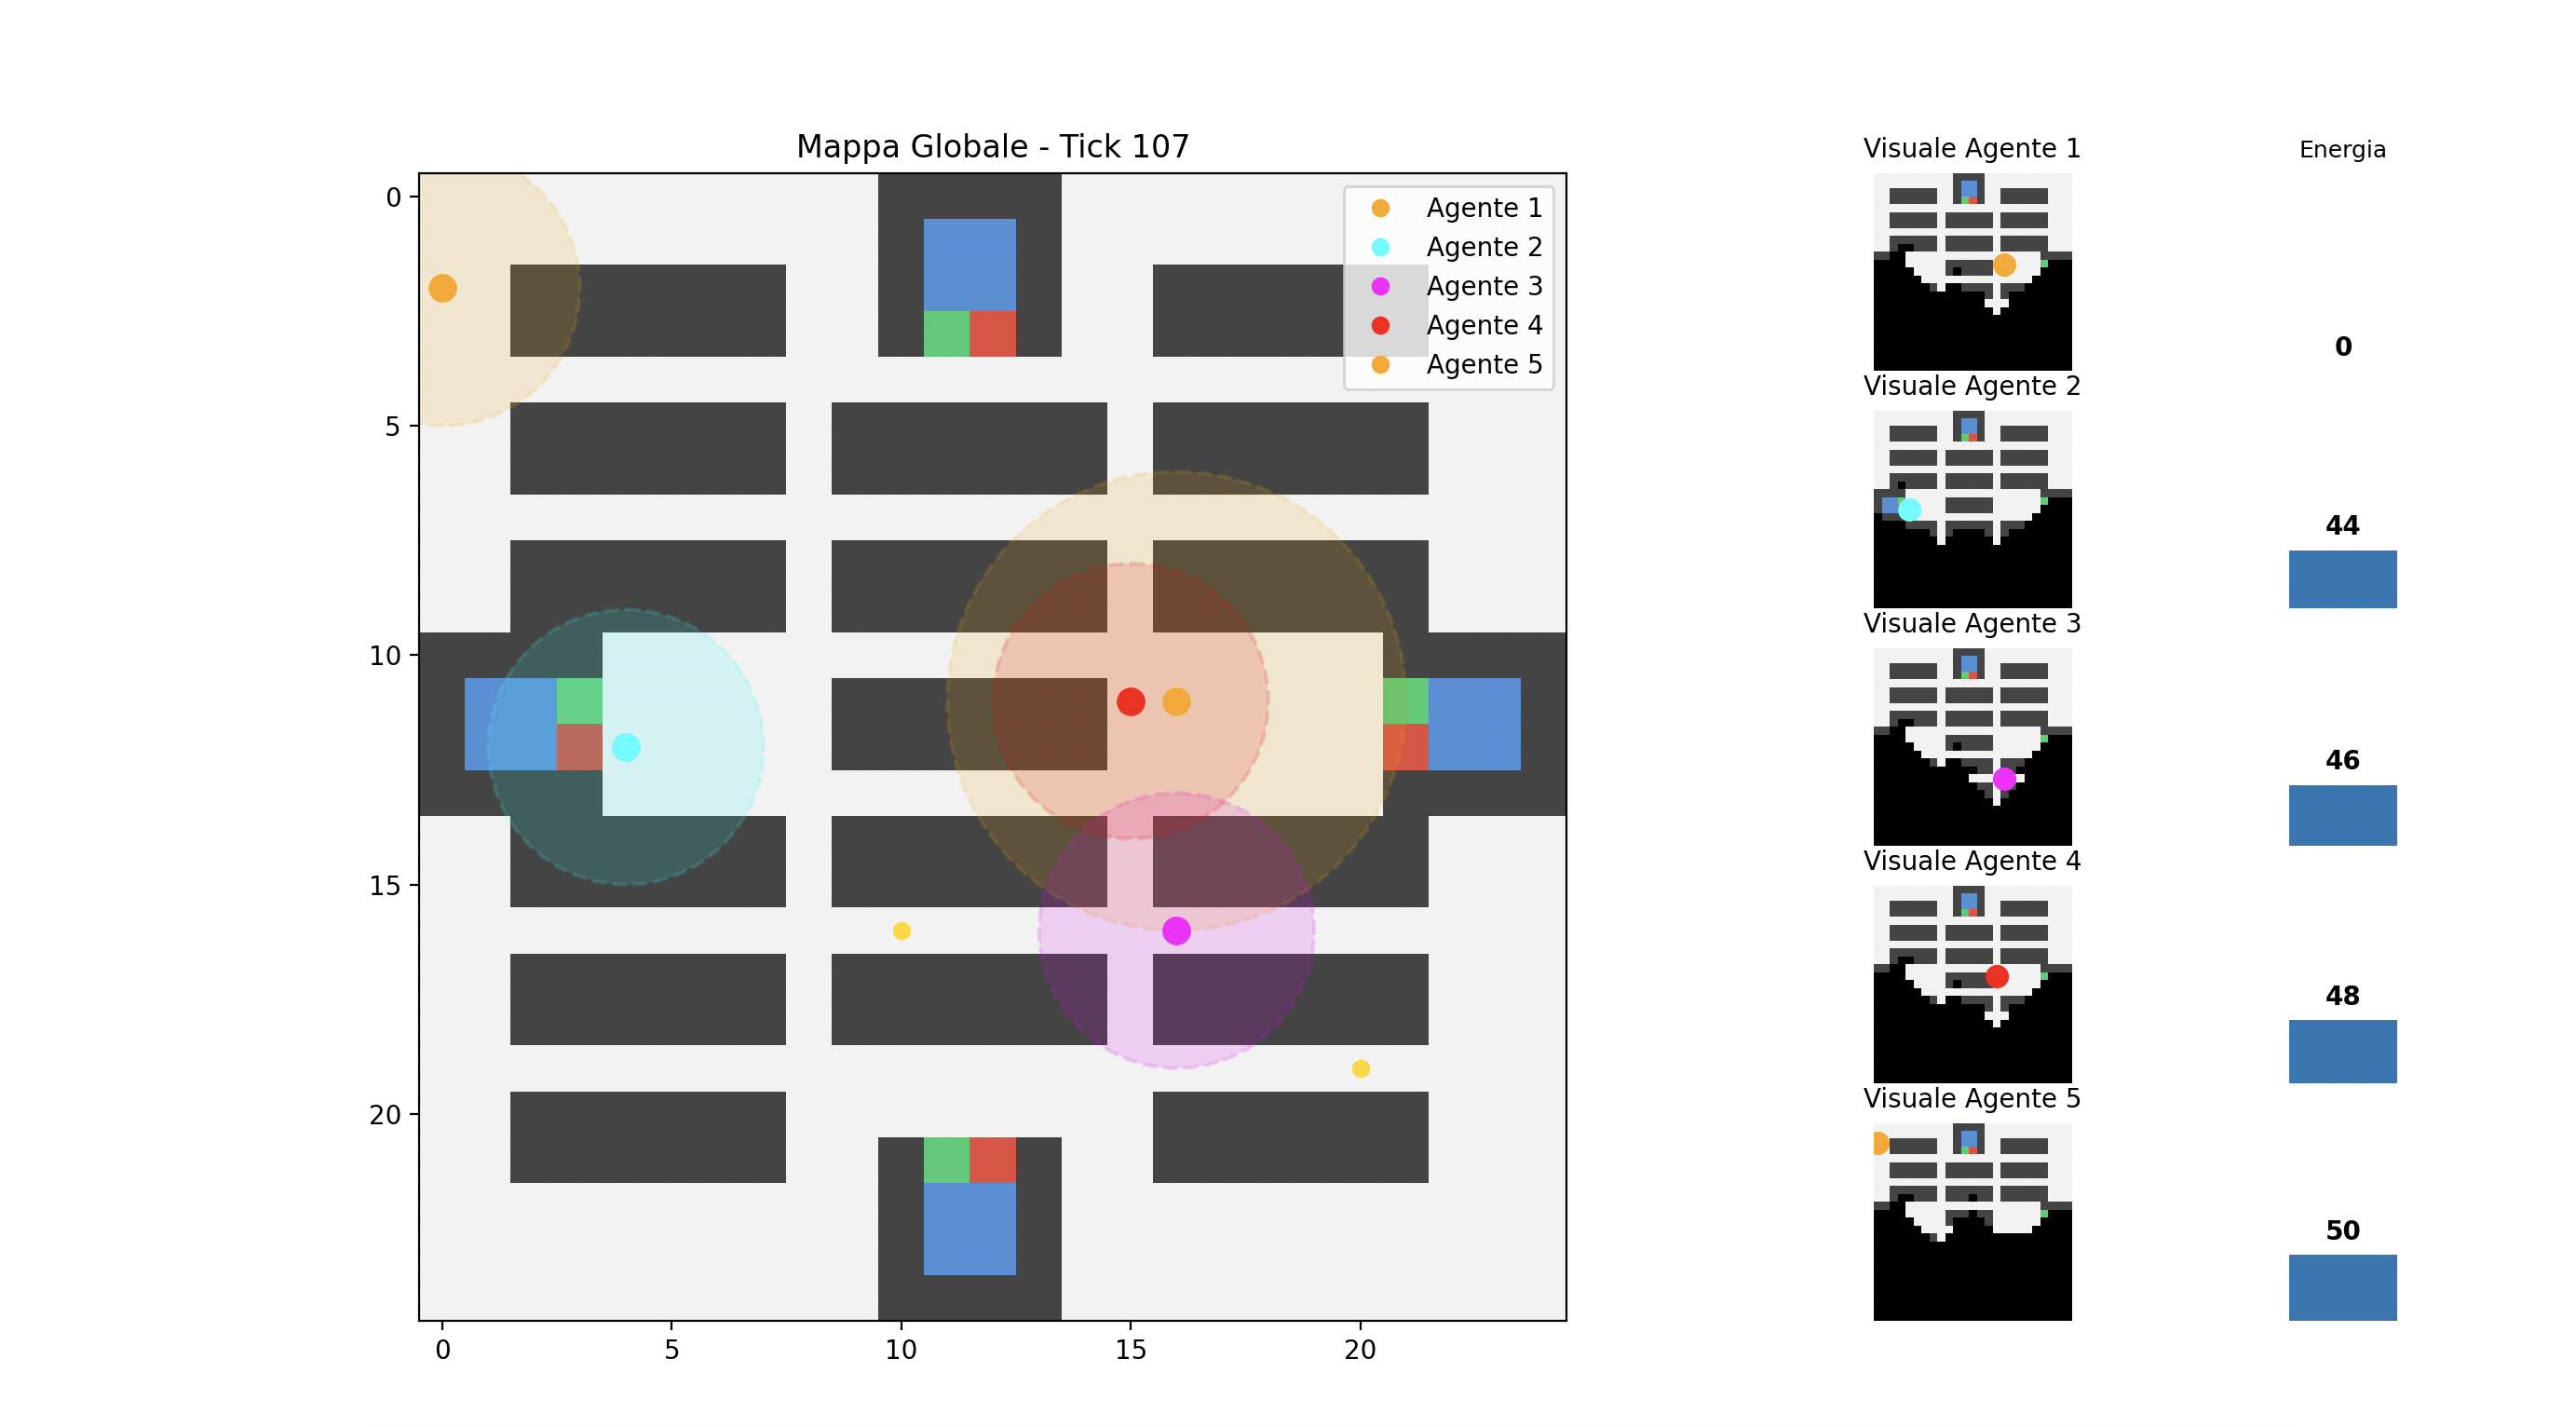
\includegraphics[width=0.9\textwidth]{simulazione.png}
    \caption{Rappresentazione visiva dell'ambiente di simulazione (generata tramite il modulo \textit{graphics.py}). Sono visibili gli agenti spazialmente distribuiti, gli ostacoli strutturali, gli oggetti da recuperare e le zone di drop-off (magazzini).}
    \label{fig:ambiente_simulazione}
\end{figure}

\vspace{0.3cm}
\noindent
All'interno di questo spazio opera una flotta di agenti autonomi, ciascuno progettato con uno stato interno e una \textbf{dotazione sensoriale specifica}. Lo stato dell'agente è definito dalle sue coordinate spaziali, da un indicatore di carico (\textit{carrying}) che segnala l'avvenuto recupero di un oggetto, e dal livello di energia residua, la quale decresce progressivamente ad ogni azione di movimento. Per interagire con l'ambiente circostante, ogni robot si avvale di due moduli percettivi:

\begin{itemize}
    \item \textbf{Sensore di Visibilità:} Opera entro un raggio predefinito e permette all'agente di acquisire informazioni topologiche (ostacoli e varchi) e rilevare target (oggetti e porte del magazzino). Il sensore rileva inoltre la presenza di altri agenti nelle celle adiacenti, informazione cruciale per attivare manovre evasive ed evitare sovrapposizioni e stalli nei colli di bottiglia.
    \item \textbf{Sensore di Comunicazione:} Abilita alla cooperazione tra agenti. Quando la distanza euclidea tra due agenti risulta inferiore al raggio di comunicazione, essi instaurano un collegamento per sincronizzare le rispettive memorie locali. Questo scambio permette di unire le porzioni di mappa esplorate e di invalidare informazioni obsolete (come la presenza di un oggetto già recuperato da un altro componente dello sciame).
\end{itemize}

\vspace{0.3cm}
\noindent
Ogni informazione captata dai sensori viene immagazzinata in una \textbf{mappa locale} individuale. Questa memoria spaziale parte da uno stato di totale incertezza e viene progressivamente popolata, fungendo da base conoscitiva fondamentale per gli algoritmi di \textit{Decision-Making} e Pathfinding del singolo agente.

\section{Processo Decisionale e Strategie di Esplorazione}
L'architettura logica che governa il comportamento degli agenti è strutturata su due moduli interconnessi, al fine di garantire un'efficace capacità di \textit{Decision-Making} e una scelta autonoma del percorso.

\subsection{Architettura Comportamentale e Macchina a Stati Finiti}
Il ciclo di vita operativo dell'agente è gestito da una Macchina a Stati Finiti (FSM). Lo stato predefinito è l'esplorazione (\textit{EXPLORE}), che guida la ricerca di nuovi target. Tale stato viene interrotto non appena il sensore individua un oggetto, innescando la transizione allo stato di recupero (\textit{REACH\_ITEM}). Acquisito il carico, l'agente passa allo stato di consegna (\textit{SEEK\_STORAGE}), calcolando la rotta ottimale verso l'ingresso del magazzino. È stata inoltre implementata una logica di emergenza (\textit{LOW\_ENERGY}) che, in caso di esaurimento critico della batteria, forza l'agente verso una zona di sosta strategica.



\begin{figure}[H]
\centering
\resizebox{0.7\textwidth}{!}{
\begin{tikzpicture}[->, >=stealth, auto, 
                    every state/.style={thick, minimum size=3cm, align=center, font=\small},
                    label node/.style={fill=white, inner sep=2pt, font=\footnotesize, align=center}]

    \node[state, initial text=Start, initial, fill=green!5]   (explore) at (0, 0)   {\textbf{EXPLORE}};
    \node[state, fill=blue!5]                                 (reach)   at (8, 0)   {\textbf{REACH\_ITEM}};
    \node[state, fill=purple!5]                               (seek)    at (8, -6)  {\textbf{SEEK\_STORAGE}};
    \node[state, fill=orange!10]                              (low)     at (0, -6)  {\textbf{LOW\_ENERGY}};
    \node[state, fill=red!15, accepting]                      (dead)    at (4, -10) {\textbf{DEAD}};

    \draw (explore) edge[bend left=20] node[label node, above] {Item Visto} (reach);
    \draw (reach)   edge[bend left=20] node[label node, below] {Item Sparito} (explore);
    
    \draw (reach)   edge node[label node,above left, pos=0.4] {Item Raccolto\\(\textit{carrying = True})} (seek);
    \draw (seek)    edge node[label node, above left, pos=0.1] {Consegnato al Magazzino\\(\textit{carrying = False})} (explore);
    
    % Transizione Emergenza Energia
    \draw (explore) edge node[label node] {Energia $\le$ 20\%} (low);

    % Transizioni verso la Morte (curvate per non tagliare il centro)
    \draw (low)     edge node[label node, above right, pos=0.4] {Energia = 0} (dead);
    \draw (seek)    edge node[label node, above right, pos=0.8] {Energia = 0} (dead);
    \draw (explore) edge[bend right=70] node[label node, left, pos=0.8] {Energia = 0} (dead);
    \draw (reach)   edge[bend left=70] node[label node, right, pos = 0.9] {Energia = 0} (dead);

\end{tikzpicture}
}
\caption{Macchina a Stati Finiti (FSM) che regola il comportamento del singolo agente.}
\label{fig:fsm_agent}
\end{figure}

\subsection{Algoritmi di Navigazione e Risoluzione dei Conflitti}
Il sistema di navigazione degli agenti si fonda su un approccio ibrido che unisce la ricerca deterministica a euristiche di memoria spaziale. 
Quando un agente acquisisce un target noto (un oggetto da raccogliere o un magazzino in cui depositare), il calcolo della traiettoria è affidato a un algoritmo di ricerca in ampiezza \textbf{(BFS)}. L'implementazione di quest'ultimo è stata specificamente adattata alla topologia dell'ambiente: l'algoritmo ignora i muri ed evita le celle di uscita quando l'agente cerca di entrare, e viceversa. 

Per governare le fasi di ricerca cieca e prevenire percorsi ciclici ridondanti, la navigazione è supportata da una memoria a breve termine (\textbf{Tabu List}). Questa struttura dati a coda circolare (con dimensione massima prefissata) tiene in memoria gli ultimi passi effettuati dall'agente, scoraggiando il ritorno sulle celle appena visitate durante la selezione stocastica delle mosse.

Infine, per garantire la fluidità del traffico in spazi ristretti, è stato sviluppato un modulo stocastico di manovra evasiva (\textbf{Collision Event}): qualora la traiettoria di un agente converga su una cella attualmente occupata da un altro agente attivo (\textit{deadlock} imminente), l'agente invalida immediatamente il percorso in memoria e successivamente calcola uno spostamento laterale o di arretramento, estraendo casualmente una direzione libera da ostacoli e da altri agenti, disimpegnando l'incrocio e permettendo allo sciame di riorganizzarsi fluidamente.

\subsection{Strategie Esplorative e Intelligenza di Sciame}
Il cuore decisionale del progetto risiede nel modulo strategico, implementato seguendo il \textbf{Design Pattern Strategy}. Tutte le logiche derivano da una classe astratta (\textit{BaseStrategy}) che fornisce gli strumenti fondamentali di mappatura. Per valutare l'impatto della cooperazione, sono state sviluppate e testate logiche a complessità crescente:

\begin{itemize}
    \item \textbf{Strategie Baseline (Random e Scout):} La \textbf{RandomStrategy} rappresenta il limite inferiore di efficienza, basandosi su un puro \textit{Random Walk} filtrato unicamente dalla Tabu List. Per ottimizzare la copertura dei corridoi, è stata introdotta la \textbf{ScoutStrategy}, la quale mantiene un vettore di direzione costante finché non rileva un ostacolo, per poi ruotare stocasticamente. Un'ulteriore evoluzione è la \textbf{ScoutStrategy2}, che adotta un approccio \textit{Frontier-Based}: l'agente interroga la memoria locale per individuare la coordinata di tipo "ignoto" più vicina, delegando al BFS la rotta per raggiungerla. Pur garantendo una rapida esplorazione individuale, queste logiche sono "cieche" rispetto ai compagni, causando un'elevata duplicazione del lavoro in scenari multi-agente.

    \item \textbf{Navigazione Perimetrale (Wall Follower):} Implementata come primo tentativo di esplorazione strutturata, si basa sulla nota "Regola della Mano Destra", costringendo l'agente a muoversi mantenendo costantemente un ostacolo sul proprio lato destro. Nonostante l'efficacia teorica nei labirinti a corridoio continuo, questa logica è stata valutata e \textbf{ufficialmente scartata}. In un ambiente logistico aperto e disseminato di ostacoli centrali (come gli scaffali), la strategia induce gravi inefficienze: gli agenti tendono a bloccarsi in cicli infiniti ridondanti (orbitando attorno a un singolo pilastro) e ignorano gli oggetti o i magazzini visibili se questi non si trovano strettamente adiacenti al muro che stanno seguendo.
    
    \item \textbf{Dispersione Fisica (Sparce Strategy):} Per ovviare all'accavallamento spaziale, questa strategia introduce una logica di repulsione a corto raggio. L'agente analizza la posizione dei compagni nel suo raggio di prossimità e calcola un "vettore di fuga" sommando le direzioni opposte ai colleghi. La mossa successiva viene scelta massimizzando il prodotto scalare tra le direzioni valide e il vettore di fuga, simulando di fatto un campo magnetico repulsivo che distribuisce uniformemente gli agenti nella stanza.
    
    \item \textbf{Intelligenza di Sciame (Swarm Explorer):} È la strategia più avanzata e collaborativa del sistema. Invece di limitarsi a schivare i compagni vicini, gli agenti si "spartiscono" in automatico le zone della mappa ancora da visitare, evitando così di esplorare tutti la stessa area. Ad ogni step, l'algoritmo valuta tutte le celle ignote della mappa, assegnando a ciascuna un costo (ovvero un livello di preferenza) basato sulla somma di tre fattori:
    \begin{enumerate}
        \item \textbf{Distanza fisica:} La distanza di Manhattan tra l'agente e la cella ignota.
        \item \textbf{Penalità Tabu (+20):} Un malus applicato se la cella rientra nella memoria a breve termine.
        \item \textbf{Interferenza dello sciame:} Il fulcro della cooperazione. Se un compagno risulta più vicino alla medesima cella ignota, viene applicata una penalità proibitiva (+100) che forza l'agente corrente a rinunciare a quell'obiettivo. Se il compagno è vicino al target (entro 8 passi), viene applicata una penalità proporzionale.
    \end{enumerate}
    L'agente seleziona il target con il costo totale minimo. Questo meccanismo garantisce un'espansione organica, in cui lo sciame si divide spontaneamente ai bivi e copre l'intera planimetria logistica nel minor numero di \textit{tick} possibili.

    \vspace{0.3cm}
Si riporta di seguito il codice \texttt{Python} che implementa la funzione di costo per l'allocazione dei target:

\begin{lstlisting}[language=Python]
best_target = None
best_score = float('inf')

for unk in unknowns:
    my_dist = position.manhattan_distance_to(unk)
    tabu_penalty = 20 if self._is_tabu(unk.x, unk.y) else 0
    teammate_penalty = 0
    
    # Calcolo dell'interferenza dello sciame
    for t in self.teammates:
        t_dist = abs(t.x - unk.x) + abs(t.y - unk.y)
        if t_dist <= my_dist:
            teammate_penalty += 100 # Compagno piu' vicino: rinuncia
        elif t_dist < 8:
            teammate_penalty += (8 - t_dist) * 2 # Compagno in avvicinamento
            
    # Funzione di costo complessiva
    score = my_dist + teammate_penalty + tabu_penalty
    if score < best_score:
        best_score = score
        best_target = unk
\end{lstlisting}
\end{itemize}


\section{Comunicazione e Coordinamento}

Il sistema implementa un modello di cooperazione decentralizzata: gli agenti comunicano tra loro scambiandosi le informazioni una volta che i raggi di comunicazione di due o più agenti si intersecano. 

\vspace{0.3cm}
\noindent
L'interazione avviene tramite un protocollo di sincronizzazione della memoria spaziale. In questo caso i due o più agenti si scambiano le informazioni delle proprie mappe locali esplorate, e di eventuali oggetti rilevati ma non recuperati. Questo scambio di dati produce tre vantaggi fondamentali per l'efficienza globale dello sciame:

\begin{itemize}
    \item Sovrapponendo le matrici delle rispettive mappe locali, gli agenti ampliano istantaneamente la propria visione dell'ambiente. Questo permette loro di scoprire la posizione dei magazzini e la conformazione degli ostacoli senza doverli esplorare fisicamente, riducendo le aree ignote.
    
    \item Condividendo lo stato di avanzamento sui target, un agente apprende tempestivamente se un determinato oggetto è già stato prelevato da un collega. Ciò permette di annullare immediatamente le rotte di recupero non più valide, risparmiando inefficienze e consumo energetico legato a viaggi a vuoto.
    
    \item L'avvenuta connessione aggiorna la percezione di prossimità dei colleghi. Questa informazione alimenta le euristiche delle logiche esplorative più complesse (come la strategia \textit{Swarm Explorer}), fornendo gli input necessari per calcolare le penalità di interferenza e permettendo agli agenti di spartirsi lo spazio inesplorato senza sovrapporsi.
\end{itemize}

% --- SEZIONE 5: SIMULAZIONE E RISULTATI ---
\section{Simulazione e Analisi dei Risultati}

\subsection{Setup Sperimentale e Metriche di Valutazione}
Per validare l'efficacia del Sistema Multi-Agente e delle strategie esplorative implementate, è stata condotta una vasta campagna di simulazioni. Per garantire la significatività statistica e appianare la varianza dovuta alla generazione stocastica, ogni configurazione è stata sottoposta a \textbf{200 iterazioni indipendenti} (100 per ciascuna mappa). I test sono stati condotti mantenendo fissa la dimensione della flotta a 5 agenti operativi. Tale scelta dimensionale verrà motivata nel prosieguo della trattazione, supportata dai risultati di un test comparativo effettuato su uno scenario a 4 agenti.

L'analisi ha monitorato tre metriche principali:
\begin{enumerate}
    \item \textbf{Tasso di Recupero (Success Rate):} Percentuale media di oggetti rilevati, raccolti e depositati.
    \item \textbf{Tempo di Completamento (Tick):} Iterazioni necessarie per l'esaurimento del task o dell'energia.
    \item \textbf{Efficienza Energetica:} Consumo medio per agente a fine iterazione.
\end{enumerate}

\subsection{Confronto prestazionale tra sciami omogenei ed eterogenei}
L'esperimento ha valutato sia configurazioni "pure" (flotte composte da agenti cloni con la medesima strategia) sia configurazioni "eterogenee" (squadre miste in cui uno o più agenti adottano una strategia minoritaria per diversificare l'esplorazione). I risultati consolidati sono riassunti nella Tabella \ref{tab:results_map_avg}.

\begin{table}[H]
\centering
\resizebox{\textwidth}{!}{
\begin{tabular}{|l|c|c|c|c|c|c|c|}
\hline
\multirow{2}{*}{\textbf{Composizione Flotta}} & \multirow{2}{*}{\textbf{Mappa}} & \multicolumn{3}{c|}{\textbf{Valori Singoli}} & \multicolumn{3}{c|}{\textbf{Medie Combinate}} \\ \cline{3-8}
 & & \textbf{Item (\%)} & \textbf{Tick} & \textbf{Energia} & \textbf{Item (\%)} & \textbf{Tick} & \textbf{Energia} \\ \hline
\multicolumn{8}{|c|}{\textit{Sciami Omogenei (Flotte Pure)}} \\ \hline
\multirow{2}{*}{ALL Wall Follower} & A & 80.80\% & 133.88 & 124.96 & \multirow{2}{*}{\textit{67.75\%}} & \multirow{2}{*}{\textit{132.84}} & \multirow{2}{*}{\textit{124.98}} \\ \cline{2-5}
                                   & B & 54.70\% & 131.79 & 125.00 & & & \\ \hline
\multirow{2}{*}{ALL Scout2}        & A & 74.60\% & 105.39 & 100.00 & \multirow{2}{*}{\textit{77.60\%}} & \multirow{2}{*}{\textbf{\textit{105.16}}} & \multirow{2}{*}{\textbf{\textit{99.77}}} \\ \cline{2-5}
                                   & B & 80.60\% & 104.92 &  99.53 & & & \\ \hline
\multirow{2}{*}{ALL Swarm Explorer}& A & 83.10\% & 169.36 & 149.35 & \multirow{2}{*}{\textit{79.70\%}} & \multirow{2}{*}{\textit{162.31}} & \multirow{2}{*}{\textit{149.68}} \\ \cline{2-5}
                                   & B & 76.30\% & 155.26 & 150.00 & & & \\ \hline
\multicolumn{8}{|c|}{\textit{Sciami Eterogenei (Es. X Specialisti + Swarm)}} \\ \hline
\multirow{2}{*}{2 Wall Follower}   & A & 84.60\% & 159.23 & 139.78 & \multirow{2}{*}{\textit{81.00\%}} & \multirow{2}{*}{\textit{157.03}} & \multirow{2}{*}{\textit{139.79}} \\ \cline{2-5}
                                   & B & 77.40\% & 154.83 & 139.80 & & & \\ \hline
\multirow{2}{*}{1 Scout2}          & A & 84.20\% & 166.17 & 139.61 & \multirow{2}{*}{\textit{83.15\%}} & \multirow{2}{*}{\textit{159.70}} & \multirow{2}{*}{\textit{139.01}} \\ \cline{2-5}
                                   & B & 82.10\% & 153.23 & 138.41 & & & \\ \hline
\multirow{2}{*}{2 Scout2}          & A & 83.70\% & 167.50 & 129.37 & \multirow{2}{*}{\textit{83.55\%}} & \multirow{2}{*}{\textit{160.10}} & \multirow{2}{*}{\textit{129.50}} \\ \cline{2-5}
                                   & B & 83.40\% & 152.70 & 129.63 & & & \\ \hline
\multirow{2}{*}{1 Wall Follower}   & A & 85.50\% & 162.37 & 144.65 & \multirow{2}{*}{\textbf{\textit{83.90\%}}} & \multirow{2}{*}{\textit{158.28}} & \multirow{2}{*}{\textit{144.48}} \\ \cline{2-5}
                                   & B & 82.30\% & 154.18 & 144.30 & & & \\ \hline
\end{tabular}
}
\caption{Risultati dettagliati per mappa con medie.}
\label{tab:results_map_avg}
\end{table}

\subsection{Analisi Critica}
Dall'analisi dei dati emergono considerazioni fondamentali sul comportamento del sistema multi-agente:

\begin{itemize}
    \item L'evidente discrepanza dei risultati ottenuti con la strategia \textit{Wall Follower} dimostra come la topologia della mappa ne influenzi fortemente l'efficienza. In ambienti caratterizzati da corridoi brevi e numerose intersezioni, come la mappa B, il tasso di successo crolla al \textbf{54.70\%}.
    \item La flotta pura \textit{ALL Scout2} registra i valori più bassi in termini di tick (105.16) e consumo energetico (99.77). Tuttavia, tale velocità è illusoria: agendo in modo egoistico, gli agenti si sovrappongono frequentemente e "svuotano" le aree centrali ignorando gli angoli, fermandosi prematuramente con un tasso di recupero sub-ottimale (\textbf{77.60\%}).
    \item La flotta pura \textit{ALL Swarm Explorer} innalza il tasso di successo sfiorando l'80\%. Il meccanismo repulsivo vettoriale distribuisce efficacemente gli agenti, ma il continuo tentativo di non intralciarsi a vicenda in corridoi stretti allunga i percorsi e i tempi di manovra (162.31 tick), gravando sul consumo energetico. Anche applicando una variante ottimizzata (\textit{4 Swarm Enhanced}), pur superando l'80\% di recupero, si registra il picco massimo di inefficienza temporale (180.97) ed energetica (174.83) a causa dell'eccessivo sovraccarico computazionale e di manovra.
    \item Il risultato più rilevante risiede nel superamento del paradigma dei "cloni". Inserendo all'interno di una base Swarm un singolo agente con logica differente (es. la configurazione mista \textit{1 Wall Follower} o \textit{2 Scout2}), il sistema raggiunge la sua \textbf{efficienza massima (83.90\% di recupero)}. L'agente anomalo agisce come elemento perturbatore: setaccia i perimetri ostici o "taglia" le traiettorie previste, fungendo da "scopritore" caotico per i colleghi senza appesantire il carico cognitivo dell'intero sciame.

\end{itemize}

\begin{figure}[H]
\centering

% --- PRIMO GRAFICO: TASSO DI RECUPERO ---
\begin{tikzpicture}
\begin{axis}[
    ybar,
    bar shift=0pt,
    width=0.95\textwidth,
    height=6.5cm,
    title={\textbf{Tasso di Recupero Oggetti (\%)}},
    ylabel={\textbf{\% Recupero}},
    ymin=60, ymax=95,
    xtick={1,2,3,4,5,6,7,8},
    xticklabels={ALL Wall, ALL Scout2, ALL Swarm, 4 Swarm, 2 Wall, 1 Scout2, 2 Scout2, 1 Wall},
    x tick label style={rotate=35, anchor=north east, font=\small},
    bar width=14pt,
    ymajorgrids=true,
    grid style={dashed, gray!50},
    nodes near coords={\pgfmathprintnumber\pgfplotspointmeta},
    every node near coord/.append style={font=\footnotesize},
    legend style={at={(0.5,-0.45)}, anchor=north, legend columns=-1, font=\footnotesize}
]
\addplot[fill=cyan!50, draw=black] coordinates {
    (1,67.75) (2,77.60) (3,79.70)
};
\addplot[fill=orange!50, draw=black] coordinates {
    (4,80.90) (5,81.00) (6,83.15) (7,83.55) (8,83.90)
};
\legend{Sciami Puri, Sciami Misti}
\end{axis}
\end{tikzpicture}

\vspace{1cm} 

% --- SECONDO GRAFICO: TEMPO ED ENERGIA ---
\begin{tikzpicture}
\begin{axis}[
    ybar=2pt,
    width=0.95\textwidth,
    height=6.5cm,
    title={\textbf{Costo Operativo: Tempo (Tick) ed Energia Consumata}},
    ylabel={\textbf{Valori Assoluti}},
    ymin=80, ymax=200,
    xtick={1,2,3,4,5,6,7,8},
    xticklabels={ALL Wall, ALL Scout2, ALL Swarm, 4 Swarm, 2 Wall, 1 Scout2, 2 Scout2, 1 Wall},
    x tick label style={rotate=35, anchor=north east, font=\small},
    bar width=8pt,
    ymajorgrids=true,
    grid style={dashed, gray!50},
    legend style={at={(0.5,-0.75)}, anchor=north, legend columns=-1, font=\footnotesize}
]
\addplot[fill=gray!40, draw=black] coordinates {
    (1,132.84) (2,105.16) (3,162.31) (4,180.97) (5,157.03) (6,159.70) (7,160.10) (8,158.28)
};
\addplot[fill=red!60, draw=black] coordinates {
    (1,124.98) (2,99.77) (3,149.68) (4,174.83) (5,139.79) (6,139.01) (7,129.50) (8,144.48)
};

\draw[very thick, dashed, black!60] (axis cs:3.5, 80) -- (axis cs:3.5, 200);

\node[anchor=north, font=\normalsize\bfseries, text=black!80] at (axis cs:2, 198) {SCIAMI PURI};
\node[anchor=north, font=\normalsize\bfseries, text=black!80] at (axis cs:6, 198) {SCIAMI MISTI};

\legend{Tempo (Tick), Energia Media}
\end{axis}
\end{tikzpicture}

\caption{In alto: Confronto del Tasso di Recupero tra le 8 configurazioni testate. In basso: Costi operativi in termini di iterazioni ed energia. Si nota come le soluzioni miste garantiscano il miglior compromesso tra successo e consumo logistico.}
\label{fig:grafici_completi}
\end{figure}

\subsection{Ottimizzazione del numero di agenti}
La scelta di impostare la flotta a 5 agenti nasce principalmente per mantenere i tempi di completamento intorno o sotto i 150 tick. Per averne la certezza, è stato fatto un test riducendo la squadra a 4 robot (\textit{4 Swarm}) e distribuendo l'energia dell'agente mancante tra quelli rimasti in gioco. I risultati, però, sono chiaramente peggiorati: il tempo medio è salito a quasi 181 tick, mancando in pieno l'obiettivo. Oltre a impiegare più tempo, i 4 agenti hanno consumato molta più energia a testa (174.83) e la percentuale di oggetti recuperati è scesa all'80.90\%. Questo conferma che 5 robot è il numero ideale per dividersi il lavoro in modo veloce ed efficiente. D'altra parte, è essenziale non eccedere con le unità per evitare il sovraffollamento degli spazi: un aumento sconsiderato degli agenti moltiplicherebbe gli stalli e le manovre evasive, rallentando pesantemente l'intera esplorazione concorrente.

% --- SEZIONE 6: CONCLUSIONI ---
\section{Conclusioni e Sviluppi Futuri}

Il presente progetto ha permesso di modellare, implementare e analizzare un Sistema Multi-Agente complesso per l'ottimizzazione logistica. Sviluppando e testando diverse euristiche di navigazione, si è dimostrato come l'impiego di una logica decentralizzata consenta a una flotta di robot di mappare un ambiente ignoto e portare a termine task di recupero senza alcun controllo centrale. 

Il risultato più significativo dell'analisi prestazionale risiede nella validazione del concetto di \textbf{Sciame Eterogeneo}. Gli esperimenti hanno provato scientificamente che l'inserimento di una percentuale di diversità algoritmica (come un agente con logica \textit{Wall Follower} all'interno di un team \textit{Swarm Explorer}) permette di rompere i cicli di stallo tipici dei sistemi cooperativi omogenei. Questo approccio ibrido ha garantito il miglior bilanciamento multicriterio, massimizzando il tasso di recupero degli oggetti senza gravare sui costi operativi di tempo ed energia.

\subsection{Sviluppi Futuri}
Nonostante la solidità dell'architettura attuale, la natura modulare del codice si presta a diverse evoluzioni concettuali per incrementare ulteriormente l'efficienza:

\begin{itemize}
    \item \textbf{Adattatività Dinamica delle Strategie:} Attualmente, un agente mantiene la medesima logica per tutta la durata della simulazione. Un'evoluzione naturale consisterebbe nell'implementare transizioni di strategia basate sullo stato interno o sul contesto. Ad esempio, gli agenti potrebbero iniziare con un approccio repulsivo (\textit{Sparce Strategy}) per massimizzare la copertura iniziale dell'area. Successivamente, al calare dell'energia sotto una soglia critica (es. 50\%), potrebbero commutare su logiche attrattive, convergendo intenzionalmente verso i compagni per fondere le mappe prima di esaurire le batterie.
    
    \item \textbf{Specializzazione di Ruolo:} Si potrebbe superare il concetto di flotta generalista introducendo classi di agenti con obiettivi asimmetrici. Inserire una quota di agenti "Scout" puri, programmati per ignorare la raccolta fisica degli oggetti (disabilitando lo stato \textit{REACH\_ITEM}) e focalizzati unicamente sull'espansione della mappa e sulla scoperta rapida dei magazzini. Questi agenti agirebbero come radar per lo sciame, comunicando le coordinate scoperte ai "Worker", i quali ottimizzerebbero le proprie traiettorie di raccolta e consegna senza disperdere energia in percorsi di ricerca cieca.
\end{itemize}

\end{document}